\documentclass[a4paper,12pt, twoside]{article}
%\documentclass[a4paper,12pt, twoside]{book}

\usepackage[papersize={210mm,297mm},tmargin=20mm,bmargin=20mm,lmargin=20mm,rmargin=20mm]{geometry}

\usepackage[utf8]{inputenc}
%https://mirror.hmc.edu/ctan/macros/latex/contrib/babel-contrib/turkish/turkish.pdf
\usepackage[english]{babel}
%\usepackage[T1]{fontenc}

\usepackage{amsmath,amssymb,mathabx}%\for eqref
\usepackage{lscape}

\usepackage{hyperref}
\hypersetup{
    colorlinks,
    citecolor=black,
    filecolor=black,
    linkcolor=blue,
    urlcolor=red}
  

%%% \usepackage{svg}
%%% https://tex.stackexchange.com/questions/122871/include-svg-images-with-the-svg-package/129854
\usepackage{graphicx}
\graphicspath{ {./figurler/} }

\usepackage[colorinlistoftodos]{todonotes}
\usepackage{fancyhdr}

\usepackage{indentfirst}
%% paragraf girintisi
\setlength{\parindent}{5ex}

\pagestyle{fancy}
\fancyhf{}
\lhead{ Kuantum Fiziği }
\chead{\thepage}
\rhead{Mesut Karakoç}
\lfoot{Akdeniz Üniversitesi}
\cfoot{}
%\rfoot{BF}

\title{Akdeniz Üniversitesi\\ Fen Fakültesi - Fizik Bölümü\\FİZ319 Kuantum Fiziği Ders Notları}

\author{\setlength{\unitlength}{6mm}
\begin{picture}(10,10)
\put(1.1,0){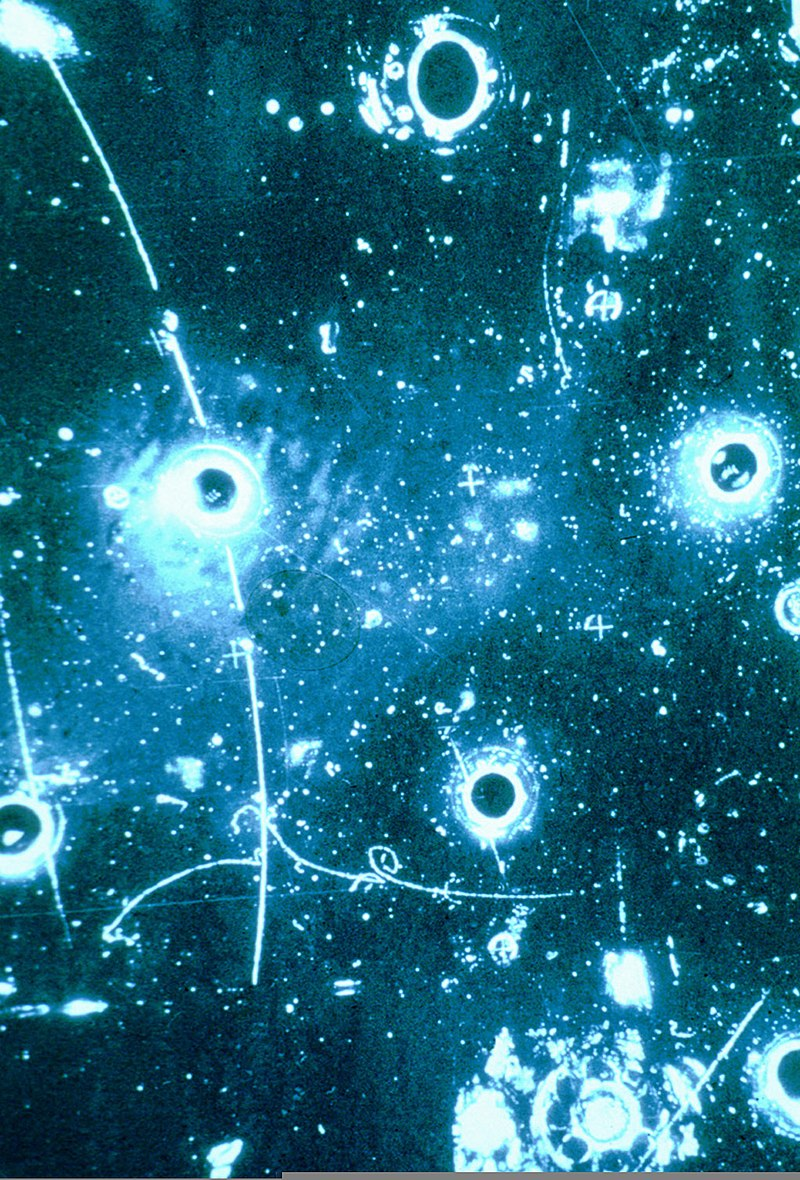
\includegraphics[width=4.5cm]{Leptonic_event_in_Gargamelle_bubble_chamber.jpg}}
\end{picture} \\ Doç. Dr. Mesut Karakoç}


\date{\today}

\begin{document}

%% Turkish babel problem
%% https://tex.stackexchange.com/questions/160385/newgeometry-doesnt-work-with-turkish-babel-package
%%\shorthandoff{=}% Make = not active any more

\maketitle

\newpage

% change name to "İçindekiler"
\renewcommand{\contentsname}{İçindekiler}
\tableofcontents{}

\listoffigures
 
\listoftables

\newpage

{
\hspace{.5\textwidth}
\begin{minipage}{.5\textwidth}
\raggedleft
For, as it has once been said, ``research is to see what everybody has seen and to think what nobody has thought." But post iacturam quis non sapit! \cite{book:Jammer}



%% Latince için
%% post iacturam quis non sapit!
%% Who is not wise after he has lost something?
%% https://quizlet.com/23756827/latin-proverbs-h-flash-cards/
\end{minipage}
}


\section{Wave-Particle Duality, 
Probability, and the 
Schrodinger Equation}

Kuantum fiziğinin doğum sürecinin 14 Aralık 1900 tarihinde başladığı kabul edilebilir. O gün Max Planck Alman Fizik Topluluğu'nun bir toplantısında ``Normal Spektrumun Enerji Dağılım Yasasının Teoremi" başlıklı makalesini sunmuştu \cite{book:EisbergResnick}. Bu makale çok ilgi görmemesine rağmen, bir elektronun enerjisinin kuantumlu olabileceğini ilk defa öne sürdüğü için önemlidir.

Kuantum fiziğinin bütünüyle sadece bu makaleyle başladığını söylemek pek doğru olmaz. On dokuzuncu yüzyılın başlarında gerçekleştirilen bazı deneyleri klasik fizik açıklamakta yetersiz kalmıştır. Bu ilk bölümde bu deneyleri ve bu deneylerin açıklanması için ortaya çıkan yeni kavramları (ışığın parçacık özelliği, maddenin dalga davranışı, fiziksel niceliklerin kuantumlanması) anlamaya çalışacağız. 


\subsection{Karacisim Işıması}

% Modern Physics
% Michael Fowler, University of Virginia
% http://galileo.phys.virginia.edu/classes/252/black_body_radiation.html
% Black Body Radiation
% http://galileo.phys.virginia.edu/classes/252/


\subsubsection{Klasik Fiziğe Göre}
On dokuzuncu yüzyılın başlarında fizikçilerin en çok ilgilendikleri konulardan birisi:
ısıtılmış cisimlerin nasıl ışıma yaptıklarıdır? Bu nedenle ısıtılmış cisimlerin ışıması üzerine bir çok deney yapılmış ve teorik olarak açıklanmaya ihtiyaç duyan bir çok deneysel veri ortaya çıkmıştır \cite{book:Sharkov}. Termal ışımalar üzerine teorik çalışmalar Gustav Kirchhoff'un 1859 yılındaki çalışmaları ile başlar \cite{book:Gasiorowicz}. 

Kirchhoff ``Işık ve ısının yayılımı ve soğurulması arasındaki ilişki" \cite{book:Jammer, Kirchhoff1859} adlı makalesinde etrafları mükemmel yansıtıcılarla sarılmış iki yayıcı ve soğurucu sonsuz paralel plakanın ısıl denge durumundaki ışınım alış verişlerini inceledi. Plakaların yayıcılık (Emitting) ve soğuruculuk (Absorbing) özelikleri için $E(\lambda, T)$ ve $A(\lambda, T)$ şeklinde iki ifade tanımladı. 

\begin{itemize}
\item $E(\lambda, T)$: yayınlanma gücü herhangi bir $T$ sıcaklığında  herhangi bir $\lambda$ dalga boyundaki ışımanın birim alan ve birim zaman başına şiddetini tanımlar ve birimi $W/m^2\equiv \frac{J}{s} \frac{1}{m^2}$'dir.
\item $E/A$ yayınlanan ışının ne kadarlık kısmının soğurulduğunu tanımlar.
\end{itemize}

Kirchhoff ortaya attığı problemdeki termal denge durumundaki levhalardan birinden yayınlanan ışınımın enerjisinin diğeri tarafından soğurulanın enerjisine eşit olması gerektiğini gösterdi ve böylece her iki plaka içinde $E/A$ oranının eşit olacağını gösterdi.

Daha sonra Kirchhoff ``kara cisim" diye adlandırdığı bütün ışık spektrumunu soğurabilen bir nesne kavramını ortaya attı ve bu nesne için $A=1$ olduğunu fark etti. Bu durumda $E(\lambda, T)$ bütün termal ışıma yapan nesneler için evrensel bir fonksiyon halini almaktadır.


%\shorthandoff{=}% Make = not active any more
\begin{figure}
\center
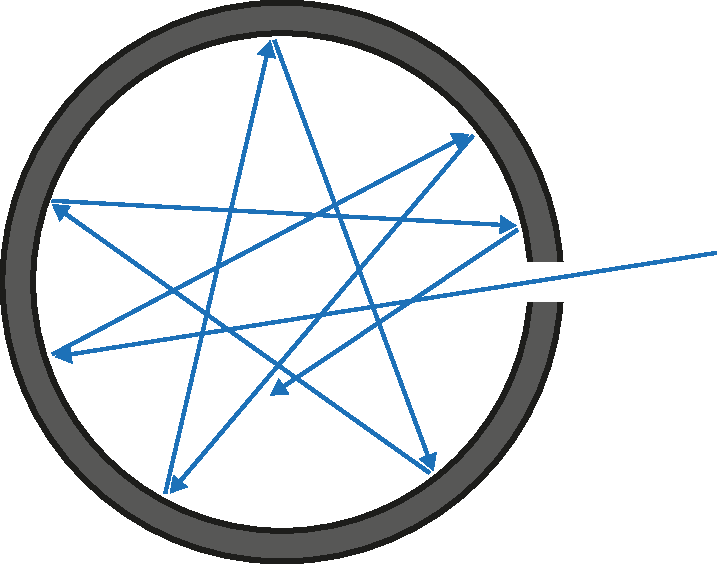
\includegraphics[scale=.5]{Black_body_realization.pdf}
\caption{Kara cisim, küre şeklindeki kovukta açılan deliktir.}
\label{fig:karacisim}
\end{figure}
%\shorthandon{=}% Make = active again

Böyle bir karacisim şekilde gibi bir küresel kovukta açılan delikle temsil edilir. Bu deliğe gelen neredeyse bütün elektromanyetik ışınlar tekrar kovuktan çıkamazlar ve kovuk duvarları tarafından soğurulurlar. Böylece kovuğun bu çok küçük deliği bütün elektromanyetik spektrumu soğuran bir kara cisim halini alır.

\begin{itemize}
\item Termodinamiğin ikinci yasısına göre yalıtılmış bir sistemin entropisi ya artar ya da ideal bir denge durumunda sabit kalır.
\end{itemize}

%% Termodinamik yasalar:
%% The zeroth law of thermodynamics states that if two thermodynamic systems each are in thermal equilibrium with a third, then they are in thermal equilibrium with each other. Accordingly, thermal equilibrium between systems is a transitive relation.

%% The first law is often formulated[1][nb 1] {\displaystyle \Delta U=Q-W.} {\displaystyle \Delta U=Q-W.} It states that the change in the internal energy ΔU of a closed system is equal to the amount of heat Q supplied to the system, minus the amount of work W done by the system on its surroundings. An equivalent statement is that perpetual motion machines of the first kind are impossible.

%% The second law of thermodynamics states that the total entropy of an isolated system can never decrease over time. The total entropy can remain constant in ideal cases where the system is in a steady state (equilibrium), or is undergoing a reversible process. In all spontaneous processes,[1] the total entropy increases and the process is irreversible. The increase in entropy accounts for the irreversibility of natural processes, and the asymmetry between future and past.[2]

%% The third law of thermodynamics is sometimes stated as follows, regarding the properties of closed systems in thermodynamic equilibrium: The entropy of a system approaches a constant value as its temperature approaches absolute zero.

Kirchhoff bu yasaya dayanarak kovuğun içinde termal ışımanın homojen olması gerektiğini ve ışıma akısının yönden bağımsız olması gerektiğini ve aynı sıcaklığa sahip herhangi bir kovuk sistemi için bu durumun geçerli olduğunu gösterdi.

Kovuğun içindeki enerji yoğunluğunun ($w(\lambda,T)$) yayınlama gücü $E$ ile olan ilişkisi aşağıdaki gibidir,
 
\begin{equation}
\label{eq:emissiveDensity}
w(\lambda,T) = \frac{4 E(\lambda,T)}{c}.
\end{equation}
%%
burada $c$ ışığın boşluktaki hızıdır. Wilhelm Wien 1894 yılında enerji yoğunluğunun (deneysel verilerin bir sonucu olarak), 
%%
\begin{equation}
\label{eq:f_lambdaT}
w(\lambda,T) = \lambda^{-5} f(\lambda T)
\end{equation}
%%
%%
\begin{figure}[hbtp]
\center
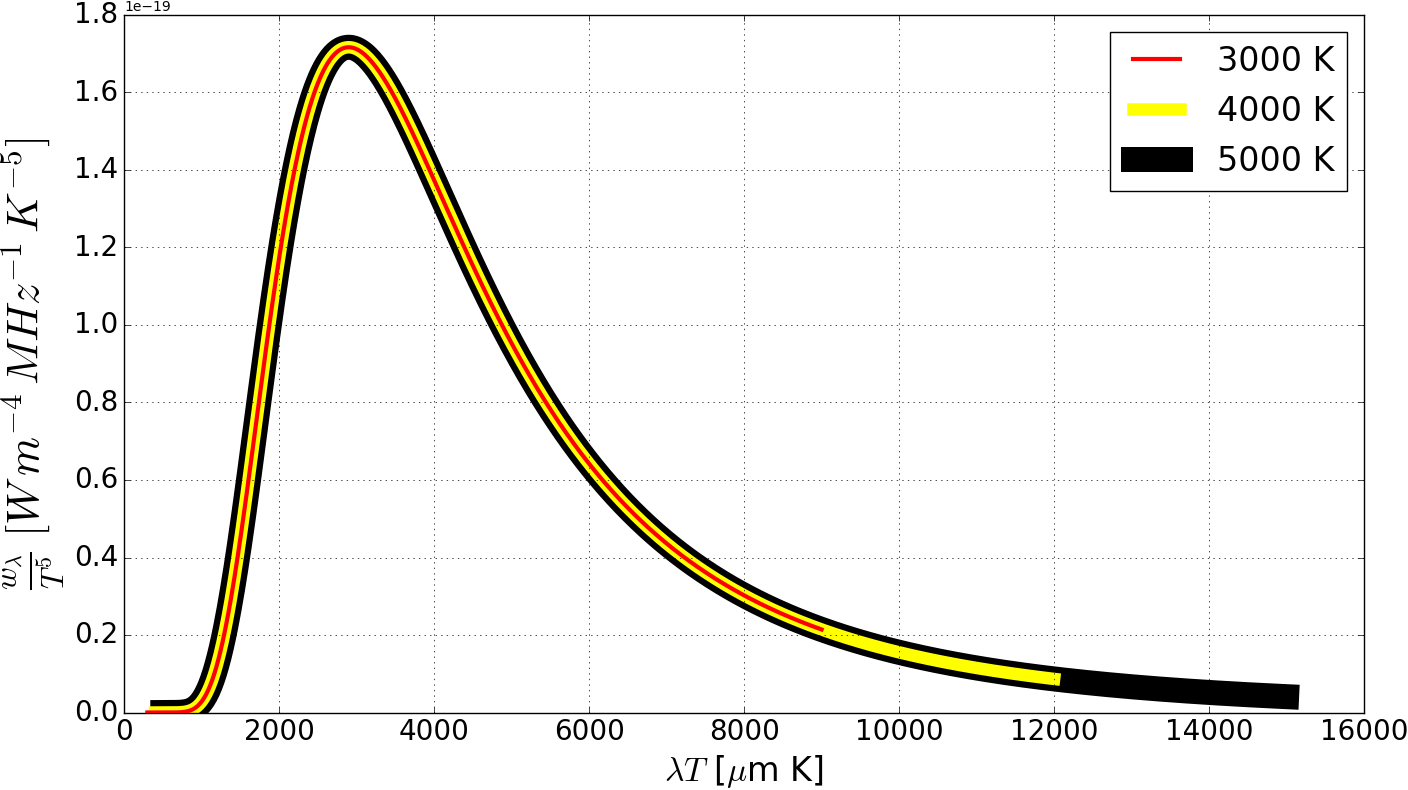
\includegraphics[scale=.4]{blackbody_spect_vs_lambdaT.png}
\caption{Denk. \ref{eq:f_lambdaT}'deki fonksiyonun varlığını gösteren spektrum.}
\label{fig:karaSpektrum_lamdaT}
\end{figure}
%%
gibi bir fonksiyon cinsinden yazılabileceğini gösterdi. Bu fonksiyonun bir benzerini frekansa bağlı olarak aşağıdaki eşitliği kullanarak yazmak da mümkündür.

\begin{equation}
\label{eq:uw_densities}
u(\nu,T) = w(\lambda,T)\left|\frac{d\lambda}{d\nu}\right| = w(\frac{c}{\nu},T)\frac{c}{\nu^2}.
\end{equation}
%%
Böylece Wien'in önerdiği tek parametreli bilinmeyen fonksiyon,
%%
\begin{equation}
\label{eq:ug_lambdaT}
u(\nu,T) = \nu^3 g(\frac{\nu}{T})
\end{equation}
%%
olarak da önerilebilir. Wien bilinmeyen bu fonksiyon için Lummer ve Pringsheim tarafından önerilen deneylere dayanarak,
%%
\begin{equation}
\label{eq:g_lambdaT}
g(\nu/T) = C e^{-\beta \nu/T}
\end{equation}
%%
formunu önermiştir ve ışıma spektrumun yüksek frekanslı (düşük dalga boylu) kısımlarını açıklamayı başarmıştır. Yine aynı fonksiyondan faydalanarak,
%%
\begin{equation}
\label{eq:wien_shift}
\lambda_{enb} = b/T 
\end{equation}
%%
%%
\begin{figure}[hbtp]
\center
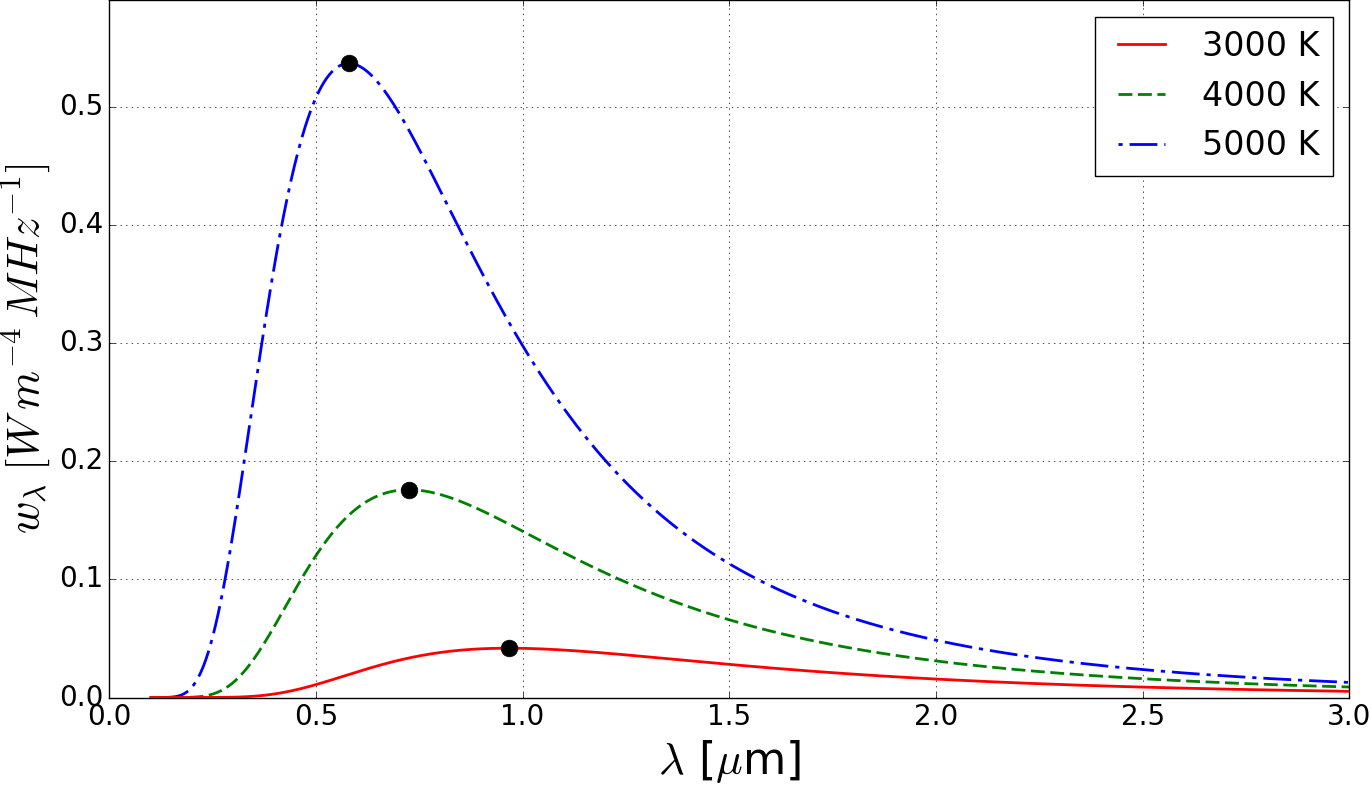
\includegraphics[scale=.4]{blackbody_spect_vs_wavelength.png}
\caption{3000, 4000 ve 5000 Kelvin sıcaklıklarındaki sistemlerin kara cisim spektrumları.}
\label{fig:karaSpektrum}
\end{figure}
%%
%%
Wien kayma yasası olarak bilinen eşitliği bulmuştur. Burada $b = 2.8977729(17)\times10^{-3}$ m K değerindedir ve biraz önce bahsedilen deneyden elde edilen bir sabittir. Bütün kara cisim spektrumları için geçerlidir. Bu yasa ile belirli bir sıcaklıkta hangi dalga boyunda en büyük ışıma şiddetinin gerçekleşeceği belirlenebilir.

Örneğin Şekil \ref{fig:karaSpektrum}'teki spektrumlar için Wien yasasından faydalanılarak Tablo \ref{tab:wien_shift}'deki değerler bulunur.
%%
%%
\begin{table}[hbtp]
\center
\begin{tabular}{|c|c|}
\hline
T ($^\circ$K) & $\lambda_{enb}\,(\mu m)$\\
\hline
3000 & 0.966 \\
4000 & 0.724 \\
5000 & 0.580 \\
\hline
\end{tabular}
\caption{\label{tab:wien_shift} Wien kayma yasası ile elde edilen dalga boyu değerleri. Şekil \ref{fig:karaSpektrum}'de spektrum eğrileri üzerinde içi dolu noktalar olarak işaretlenmişlerdir.}
\end{table}
%%

Wien'in modeli yüksek frekanslarda deneyle uyumlu olmasına karşın düşük frekanslarda bu başarıyı yakalayamamıştır. Ek olarak Wien'in modeli klasik fiziğin temel bazı varsayımlarını göz önüne almamamıştır. J. W. S. Rayleigh klasik fizikteki enerjinin eş bölüşümü teoremini ve elektromanyetik dalgaların kovuk içerisindeki normal modlarını hesaba katarak,
%%
% eş bölüşüm teoremi
% https://en.wikipedia.org/wiki/Equipartition_theorem#cite_note-4
%
\begin{equation}
\label{eq:Rayleigh}
u(\nu, T) = \frac{8 \pi \nu^{2}}{c^{3}} k_{B} T
\end{equation}
sonucuna ulaşmıştır. Burada $k_B = 1.38064852 \times 10^{-23}$ J/K, Boltzmann sabitidir ve enerjinin eş bölüşüm teoremine göre $k_B T$ serbestlik derecesi başına ortalama enerjidir. Elde edilen bu dağılım Rayleigh-Jeans dağılımı olarak bilinir. Jeans'in katkısı Rayleigh'in hesaplarında yaptığı bir düzeltmeden kaynaklanmaktadır. Rayleigh-Jeans dağılımı Wien dağılımının aksine yüksek frekanslarda başarısızdır. Ek olarak bütün frekanslar üzerinden alınan integral sonucunda elde edilen kovuk içindeki toplam enerji yoğunluğu ıraksar ve sonsuz değer verir, böylece fiziksel açıdan doğru olmayan bir sonuç elde edilmiş olur.






\subsubsection{Planck Dağılımı ve Kuantumlu Enerji Kavramı}

Planck, Wien ve Rayleigh-Jeans dağılımlarını dikkate alarak deneysel eğriyi çok iyi açıklayan,
%%
\begin{equation}
\label{eq:Planck}
u(\nu, T) = \frac{8 \pi h}{c^{3}} \frac{\nu^{3}}{e^{\frac{h \nu}{k_{B} T}} - 1}
\end{equation} 
%%
dağılım formülünü elde etmiştir. Burada $h$ daha sonra çok ünlenen fakat Planck tarafından sadece deneysel ve teorik eğriyi birbirine uydurabilmek için eklenmiş bir serbest parametredir. Serbest parametrenin(!) değerinin $h=6.626070040 \times 10^{-34}$~J~s olduğu bulunmuş ve adına Planck sabiti denmiştir.Planck'ın elde ettiği dağılım ifadesi $\frac{h\nu}{k_B T}<<1$ için Rayleigh-Jeans dağılımına indirgenirken, $\frac{h\nu}{k_B T}>>1$ için Wien dağılımana indirgenmektedir.

\begin{figure}[hbtp]
\begin{minipage}{0.49\textwidth}
\center
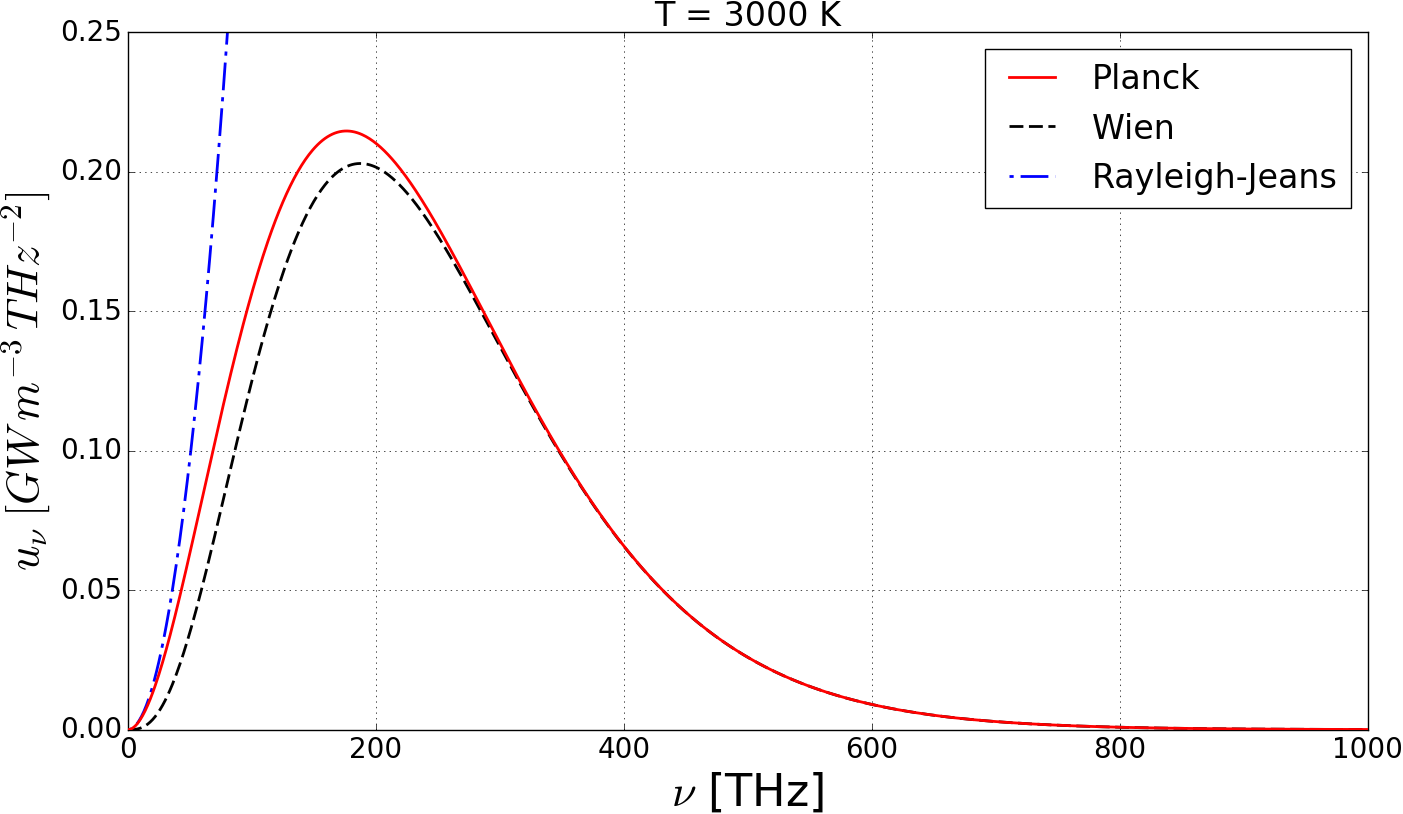
\includegraphics[scale=.22]{blackbody_spect_vs_frequency_diff_models.png}
\caption{Üç farklı modelle elde edilen kara cisim ışıma spektrumlarının frekansa göre davranışı.}
\label{fig:karaSpektrum_nu}
\end{minipage}
\hspace{12pt}
\begin{minipage}{0.49\textwidth}
\center
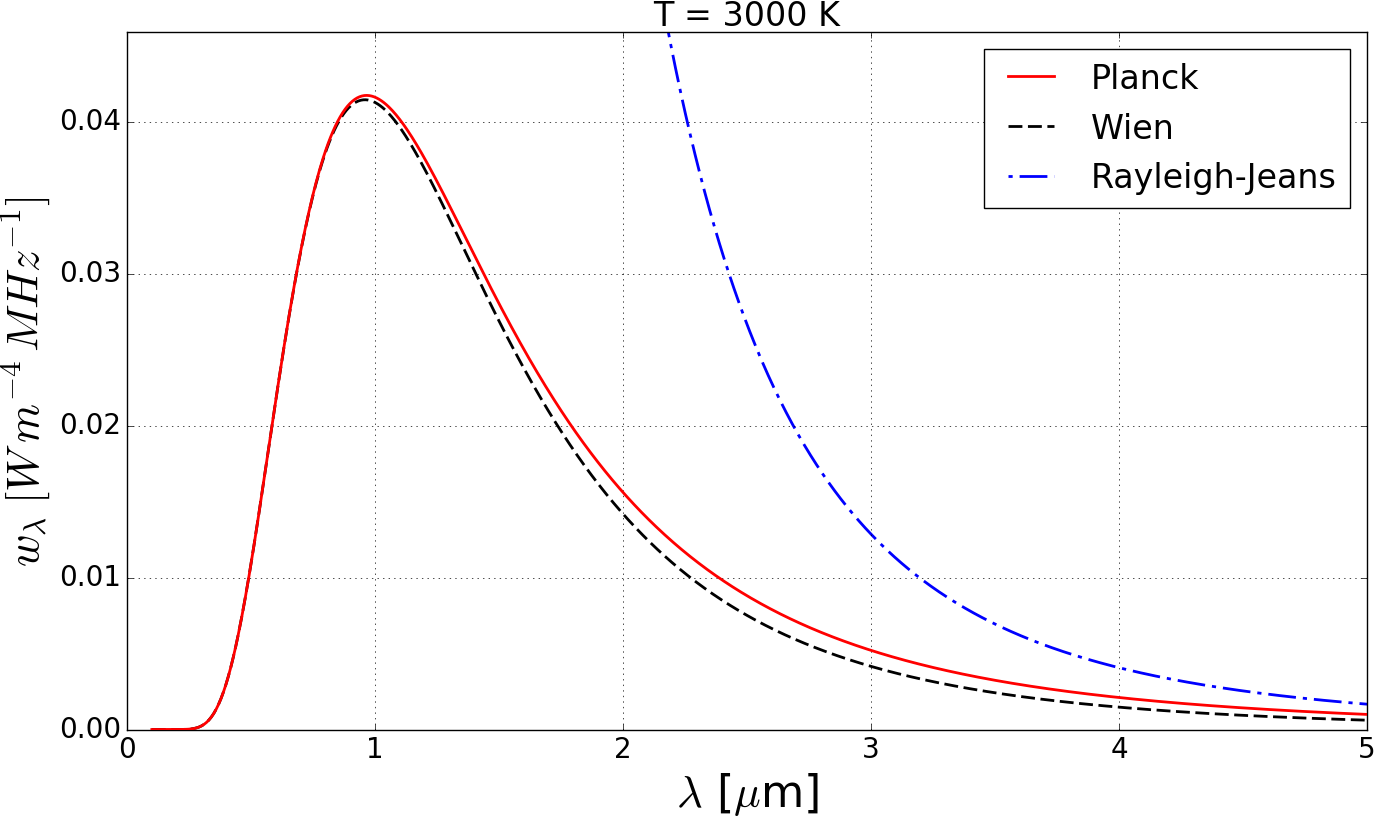
\includegraphics[scale=.22]{blackbody_spect_vs_wavelength_diff_models.png}
\caption{Üç farklı modelle elde edilen kara cisim ışıma spektrumlarının dalga boyuna göre davranışı.}
\label{fig:karaSpektrum_lambda}
\end{minipage}
\end{figure}

Planck ilk önceleri bu ifade için teorik bir temel kuramasa da daha sonra, kovuğun duvarlarındaki ışınımın yayılma ve soğurulma dinamik dengesini izah edebilmek için kovuğun duvarlarının basit salınıcılar (osilatör) gibi davrandığını ortaya atmıştır. Bu düşünceyi ortaya atarken önemli bir varsayımda bulunmuştur: ``herhangi bir  $\nu$ frekanslı ışınımın sadece $\large \boldsymbol{E=h\nu}$ enerjili paketler (kuanta) halinde yayılabilir veya soğurabilir".

Boltzmann dağılımı ile kara cisim kovuğu içindeki ortalama enerji,
%%
\begin{equation}
\label{eq:AvE_Boltzmann}
\overline E =\frac{\int \limits_0^\infty E P(E) dE}{\int \limits_0^\infty P(E) dE} 
\end{equation} 
%%
ifadesi ile hesaplanabilir. Burada $P(E)$ basit harmonik salınıcıların $E$ enerjisine sahip olma olasılığını tanımlayan Boltzmann dağılımıdır ve
%%
\begin{equation}
\label{eq:Boltzmann}
P(E) = \frac{e^{-E/k_BT}}{k_BT}
\end{equation} 
%%
olarak tanımlanır. Planck $E$'nin sürekli bir değişken değilde izinli ve kesik değerlere sahip olmasını gerektiğini düşündüğünden, $n = 0, 1, 2, \dots$  olmak üzere, Denk. \ref{eq:AvE_Boltzmann},
%%
\begin{equation}
\label{eq:Boltzmann_Planck}
\overline E =\frac{\sum \limits_{n=0}^\infty E P(E)}{\sum \limits_{n=0}^\infty P(E)} 
\end{equation}
%%
olarak yazılabilir. Böylece, herhangi bir radyasyon yayılımı ve soğurulması $E=nh\nu$ enerjili değerler alabildiğine göre,
%%
\begin{equation}
\label{eq:Boltzmann_Planck}
\overline E =\frac{\sum \limits_{n=0}^\infty nh\nu \frac{e^{-E/k_BT}}{k_BT}}{\sum \limits_{n=0}^\infty \frac{e^{-E/k_BT}}{k_BT}} 
\end{equation}
%%
sonucuna ulaşılır. Gerekli matematiksel işlemler tamamlandığında \cite{book:EisbergResnick} kovuk içi basit salınıcıların (harmonik osilatörlerin) ortalama enerjisi,
%%
\begin{equation}
\label{eq:Planck_Av_E}
\overline E = \frac{h\nu}{e^{\frac{h \nu}{k_{B} T}} - 1}
\end{equation}
%%
olarak bulunur. Elde edilen bu sonuç birim hacimdeki harmonik osilatör sayısı ile çarpıldığında Denk. \ref{eq:Planck}'deki Planck dağılımı elde edilmiş olur. 

Şekil \ref{fig:karaSpektrum_nu} ve \ref{fig:karaSpektrum_lambda}'te sürekli çizgiyle çizilen dağılım Planck dağılımıdır ve deneysel verileri en iyi açıklayan dağılımdır. Ek olarak Planck enerji yoğunluğu dağılımının bütün frekanslar üzerinden integrali alındığında Rayleigh-Jeans gibi ıraksamaz ve sonlu bir değerde kalır. Integral ve sonucu aşağıdaki gibidir.
%%
\begin{equation}
\label{eq:Planck_U_total}
U(T) = \frac{8 \pi h}{c^{3}} \int\limits_0^\infty d\nu \frac{\nu^{3}}{e^{\frac{h \nu}{k_{B} T}} - 1} = a T^4
\end{equation}
%%
Eğer integral yayınım gücü yoğunluğu üzerinden alınmış olsaydı sonuç,
%%
\begin{equation}
\label{eq:Planck_E_total}
E(T) = \sigma T^4
\end{equation}
%%
olurdu. Her iki ifade de karacisim ışınımı için benzeri bir sonucu ifade etmektedir ve Stefan-Bolzman yasası olarak bilinmektedir: ``bütün ışıma spektrumu üzerinden alınan integral sonucu elde edilen ışıma enerji yoğunluğu veya ışıma yayınım gücü sıcaklığın dördüncü kuvvetiyle doğru orantılıdır". Her iki ifadedeki sabitlerin değerleri,
%%
\begin{eqnarray}
\label{eq:stefan_boltzman}
\sigma &=&  5.670367(13) \, \times 10^{-8}\ \textrm{W}\,\textrm{m}^{-2}\,\textrm{K}^{-4} \\
a &=& 4\frac{\sigma}{c} \nonumber
\end{eqnarray}
%%
olarak verilir ve $\sigma$ Stefan-Boltzmann sabiti \cite{codata:stefan_boltzman} olarak adlandırılır.


Planck neden bu şekilde kesikli bir davranışın gerçekleştiğine bir açıklama getiremedi ve bilinmeyen bir neden kovuk duvarlarındaki atomların paketler (kuantlar) halinde kesikli enerjiler yayınladıklarını öne sürdü. Bilinmeyen nedenin açıklaması fotoelektrik etkinin Einstein tarafından çalışılmasıyla ortaya çıktı.

Günlük hayatımızda ışığın kesikli veya parçacıklı doğasını görememiz doğaldır. Örneğin, beyaz ışık yayan ve 5 Watt'lık tasarruflu bir ampulden gözümüze 400 nm (mor) ve 700 nm (kırmızı) dalga boyu aralığında bir çok ışık gelmektedir ({\it \href {https://upload.wikimedia.org/wikipedia/commons/2/25/Electromagnetic-Spectrum.svg}{elektromanyetik spektrum web link}}). Ampülden gelen bütün ışığın en küçük dalga boyuna yani en fazla enerjiye sahip olduğunu varsayalım. Bu durumda bir tek ışık paketinin sahip olacağı enerji,
%%
\begin{equation}
\label{eq:example_light_quanta01}
h\nu = h c/\lambda = \frac{6.63\times10^{-34}\,\,3\times10^{8}}{400\times10^{-9}} \eqsim 5\times 10^{-19} J 
\end{equation}
%%
olur. Bu çok küçük bir enerji miktarıdır. 5 Watt'lık tasarruflu ampülün bir saniyede yayınlayacağı ışık paketi sayısı ise,
%%
\begin{equation}
\label{eq:example_light_quanta02}
N = \frac{5\,J/s}{5\times10^{-19}\,J} \eqsim 10^{19} paket/s
\end{equation}
%%
olur.Bu miktarda paketin bir saniyede insan tarafından tek tek sayılması mümkün değildir!

% CMB: Cosmic Microwave Background
% https://wmap.gsfc.nasa.gov/universe/bb_cosmo_fluct.html
% https://en.wikipedia.org/wiki/Chronology_of_the_universe
% https://simple.wikipedia.org/wiki/Cosmic_microwave_background_radiation

% YOUTUBE
% https://www.youtube.com/watch?v=LnmCsNQsR68
% https://www.youtube.com/watch?v=HnBZf1RfB-w



\subsection{Fotoelektrik Etki}

1860'larda Maxwell ünlü Elektrik ve Manyetik alan denklemlerini yazdı, bu denklemer elektrik yükünün olmadığı bir yerde 
%%
\begin{align}
\label{eq:maxwell}
  \vec \nabla \cdot \vec{E} &= 0 \quad & \nabla \times \vec{E} &=              -\frac{\partial\vec B}{\partial t}, \\
    \vec \nabla \cdot \vec{B} &= 0 \quad & \nabla \times \vec{B} &= \mu_0\varepsilon_0 \frac{\partial\vec E}{\partial t}.
\end{align}
%%
şeklini alırlar. Bu denklemlerden faydalanarak Elektrik ve Manyetik alanının zamanla davranışını Elektromanyetik (EM) dalga olarak aşağıdaki denklemlerle tanımladı. 
%%
\begin{align}
\label{eq:maxwell_EM_wave}
  \mu_0\varepsilon_0  \frac{\partial^2   \vec{E}}{\partial t^2} - \nabla^2   \vec{E} = 0 \\
  \mu_0\varepsilon_0 \frac{\partial^2   \vec{B}}{\partial t^2} - \nabla^2 \vec{B} = 0
\end{align}
%%
Işığın da bu denklemlere uygun davranış gösteren EM dalgaları olduğu biliniyordu. Denk. \ref{eq:maxwell_EM_wave} dalga denklemlerinin çözümüyle belirlenen bu EM dalgaları boşlukta, 
%%
\begin{align}
\label{eq:EM_waves}
\vec E = \vec E_0 \sin(kz-\omega t),\hspace{36pt} \vec B = \vec B_0 \sin(kz-\omega t), 
\end{align}
%%
ifadeleri ile tanımlanırlar. Burada $k=2\pi\lambda$ dalga sayısı ve $\omega=2\pi\nu$ açısal frekanstır. EM dalgaları temsili olarak aşağıdaki şekildeki gibi ilerler ve enerji taşırlar.
%%
\begin{figure}[hbtp]
\center
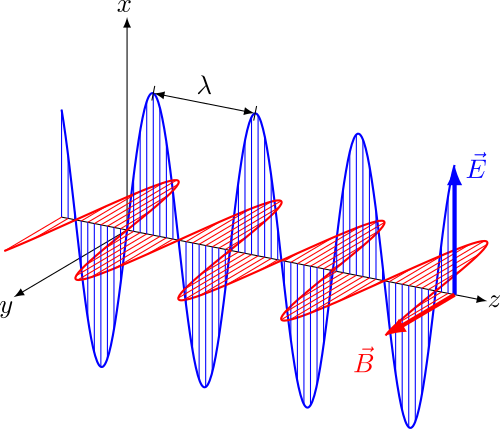
\includegraphics[scale=1.2]{EM_wave_poynting_vector.png}
\caption{$+z$ yönünde ilerleyen düzlem EM dalgalar.}
\label{fig:poynting}
\end{figure}
%%
EM dalgalarının taşıdığı enerjinin akısı matematiksel olarak ise Poynting vektörü ile tanımlanır. Yukarıdaki düzlem dalgalar için,
%%
\begin{align}
\label{eq:poynting_vec}
\vec S = \frac{1}{\mu_0}\vec E \times \vec B
\end{align}
%%
genel tanımından yola çıkarak,
%%
\begin{align}
\label{eq:poynting_plane_wave}
\vec S = \frac{1}{\mu_0} E_0 B_0 \sin^2(kz-\omega t)\hat z
\end{align}
%%
olarak bulunur. Poything vektörü birim alan başına aktarılan gücü ($W/m^2$) veya birim alan başına birim zamanda aktarılan enerjiyi ($J/s/m^2$) tanımlar. Eğer $x-y$ düzlemine paralel $z$ eksenine dik $A$ alanına sahip bir dedektör yüzeyine aktarılacak gücü hesaplamak istersek,
%%
\begin{align}
\label{eq:poynting_power1}
P = S A
\end{align}
%%
ile hesaplayabiliriz. EM dalgasının elektrik ve manyetik alan bileşenlerinin genlikleri arasında $B_0 = E_0/c$ bağıntısı olduğunu da hatırlayarak,
%%
\begin{align}
\label{eq:poynting_power2}
P = \frac{1}{\mu_0 c} E_0^2 A \sin^2(kz-\omega t)
\end{align}
%%
ile dedektöre aktarılan gücü hesaplayabiliriz. Böylece klasik olarak ışığın bir yüzeye aktarabileceği gücün (veya şiddetin $I = P/A$) elektrik veya manyetik alanın genliğinin karesiyle orantılı olduğu görülür.

Fakat, 1887'de Heinrich Hertz onu izleyen diğerleri tarafından gerçekleştirilen fotoelektrik etki deneyleri ışığın EM dalga davranışına aykırı sonuçlar ortaya koydu.
%%
\begin{figure}[hbtp]
\center
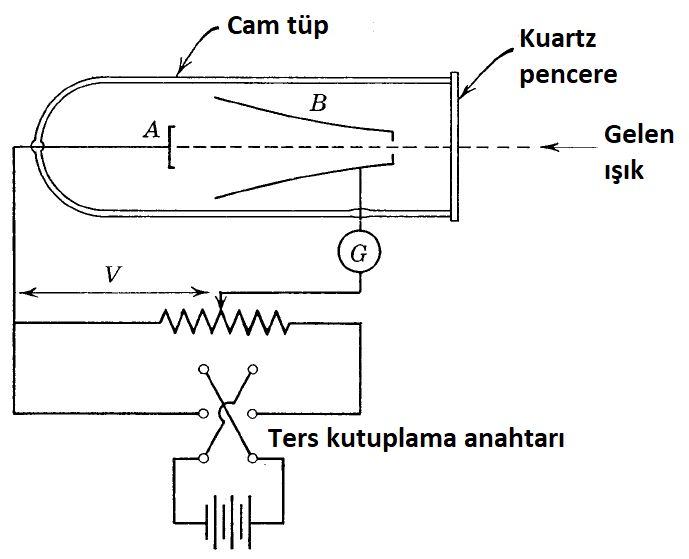
\includegraphics[scale=.5]{fotoeletrik_deney_devresi.png}
\caption{Hertz tarafından kullanılan deney düzeneğinin şeması \cite{book:EisbergResnick}.}
\label{fig:fotoeletrik_devresi}
\end{figure}
%%
Deneyde basitçe, A metal plakasına gelen tek renkli ışık eğer elektron koparabilirse ve bu koparılan elektron B plakasına ulaşabilirse $G$ ampermetresinde bir akım okunmaktadır. Böyle bir deney düzeneğinden klasik EM teoremine göre elektronların koparılabileceği ve dolayısıyla fotoelektrik etkinin izah edileceği düşünülebilir. Buna göre klasik fiziğin fotoelektrik etki için tahminleri \cite{book:KraneS} aşağıdaki gibi özetlenebilir.
%%
\begin{itemize}
\item {\bf Koparılan elektronların sahip olabileceği en büyük kintetik enerji ışığın şiddetiyle orantılı olmalıdır:} Işığın şiddeti arttıkça $E$ artmalı, $E$ arttıkça $I=P/A$ artmalıdır. Böylece bir elektrona aktarılan enerji artmalıdır.

\item {\bf Fotoelektrik etki ışığın frekansından veya dalga boyundan bağımsızdır:} Işığın şiddeti yeterliyse frekansı ne olursa olsun elektron koparılabilmelidir.

\item {\bf Işık $A$ plakasına vardıktan sonra saniye mertebesindeki sürelerde plakadan elektron yayınlanır:} $\Delta E/\Delta t = P_{ort}$ ifadesinden bir elektronu koparmak için ne kadar süre harcanması gerektiği hesaplanabilir. Burada $\Delta E$ elektron koparmak için gerekli enerji, $P_{ort}$ gönderilen ışığın ortalama gücü ve $\Delta t$ elektronun koparılma süresidir.
\end{itemize}

%%
\begin{figure}[hbtp]
\center
\begin{minipage}{0.45\textwidth}
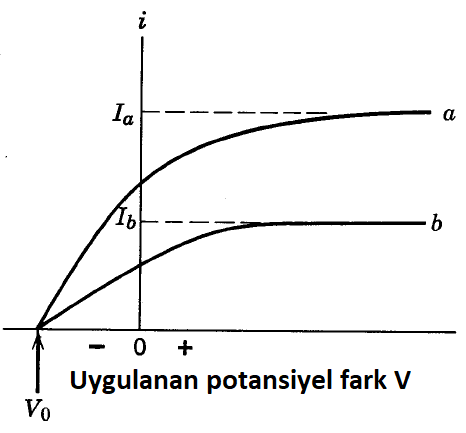
\includegraphics[scale=.5]{fotoeletrik_enyuksek_KE.png}
\caption{Fotoelektronların (fotoelektrik etkiyle koparılan elektron) sahip olabileceği en büyük kinetik enerjinin ölçümü \cite{book:EisbergResnick}.}
\label{fig:fotoeletrik_elektron_KE}
\end{minipage}
%%%
\hspace{24pt}
%%%
\begin{minipage}{0.45\textwidth}
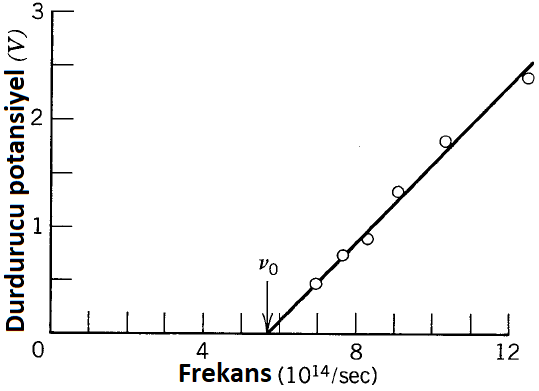
\includegraphics[scale=.5]{fotoeletrik_nu0_workFunction.png}
\caption{Işık gönderilen plakanın cinsine bağlı olarak belirli bir frekans değerinin altındaki değerlerde fotoelektron koparılamaz \cite{book:EisbergResnick}.}
\label{fig:fotoeletrik_workfunction}
\end{minipage}
\end{figure}

Klasik EM teorinin önerilerine rağmen deneylerde gözlenen sonuçlar aşağıdaki gibidir.
%%
\begin{itemize}
\item {\bf Belirli bir frekanstaki veya dalga boyundaki ışık ile koparılan bir elektronun en yüksek kinetik enerjisinin ışığın şiddetiyle bağlantısı yoktur:} Şekil \ref{fig:fotoeletrik_elektron_KE}'e göre $i$ akım ekseni ışığın şiddeti arttıkça yayınlanan elektron sayısının arttığının bir ölçüsüdür. Fakat her iki farklı şiddetteki ışığın ortak noktası frekanslarının aynı olmasıdır ve bir elektrona aktarabildikleri enerji aynıdır.

\item {\bf Eğer ışığın frekansı belirli bir değerin altındaysa fotoelektrik etki gerçekleşmez:} Deney düzeneğindeki metal plakanın cinsine bağlı olarak ışığın frekansı yetersizse, şiddeti ne olursa olsun ışık elektron yayınlanmasını sağlayamaz (bkz. Şekil \ref{fig:fotoeletrik_workfunction}).

\item {\bf Işık metal plakaya ulaştıktan $10^{-9}$~s sonra, neredeyse hiç zaman geçmeden, fotoelektron salınımı gerçekleşir:} Bu durum klasik EM dalga teorisinin tahmin ettiği saniye mertebesiyle çelişmektedir.

\end{itemize}

Einstein 1905 yılında Planck'ında fikirlerinden faydalanarak ışığın dalga paketleri halinde,
\begin{equation}
\label{eq:photon_E}
E = h\nu
\end{equation}
var olabileceklerini ortaya attı. Planck'da kesikli enerjili ışımaları önermişti fakat Plank'a göre siyah cismin duvarlarından salınan termal ışımalar $h\nu$  enerjisiyle salındıktan sonra tekrar bir su dalgası gibi yayılmaktaydılar. Einstein ise salınan bu ışık paketlerinin (light quanta) dalga gibi yayılmak yerine birer parçacık gibi davrandıklarını iddia etmiştir. Bu parçacığa daha sonraları foton adı verilmiştir.

Foton adlı bu parçacıklar $h \nu$ enerjisi taşımakla beraber boşlukta ışık hızında hareket ederler ve bu yüzden Einstein'in bir başka teorisine göre (özel görelilik) hareket ederler. Bu teoriye uyduklarına göre kütle sahibi olamazlar aksi takdirde ışık hızına ulaştıklarında sonsuz enerjili olmaları gerekir. Bu teoreme göre fotonlar aynı zamanda $p = E/c$ momentumu taşırlar. Böylece kütleli parçacıklara benzer davranışlar göstermiş olurlar.

Einstein metal plakaya gelen fotonlardan fotoelektron koparanların enerjilerinin fotoelektronlar tarafından tamamen soğurulduğunu varsaydı ve bunun denklemini enerji korunumundan,
%%
\begin{equation}
\label{eq:photon_E}
h\nu = \frac{1}{2}m_e v^2 + W
\end{equation}
olarak tanımladı. Bu formülden anlaşıldığı üzere $\nu$ frekanslı fotonun enerjisinin bir kısmı fotoelektronu metal yüzeyden koparmak için harcanır ve iş fonksiyonu ($W$) olarak adlandırılır. Geri kalanı ise fotoelektronun kinetik enerjisini oluşturur. Bu kinetik enerji sayesinde fotoelektron diğer plakaya ulaşır ve fotoelektrik etki kaynaklı elektrik akımı oluşur.

Bu denklem ile Einstein fotoelektrik etkinin üç sonucunu da izah etmiş oldu.

\begin{itemize}
\item Denklem \ref{eq:photon_E} ışığın şiddetinden bağımsızdır, böylece Şekil \ref{fig:fotoeletrik_elektron_KE}'deki $V_0$ durdurma potansiyelinin $K_{enb}=-eV_0=h\nu - W$ eşitliğinden en yüksek kinetik enerjiyi vereceği açıktır.

\item Aynı denklem $\frac{1}{2}m_e v^2 = h\nu - W$ olarak yeniden yazılırsa bir fotonun Şekil \ref{fig:fotoeletrik_workfunction}'deki gibi bir en küçük $\nu_0$ frekansına sahip olması gerektiği anlaşılır. Aksi takdirde fotoelektron yayılımı gerçekleşmez.

\item Fotonlar $E=h\nu$ enerjili ve  $p= E/c = h\nu/c = h/\lambda$ momentumlu bir parçacık gibi davrandıklarından, metal yüzeyindeki bir elektronla etkileşmeleri ve elektronu metal yüzeyden koparmaları neredeyse anında gerçekleşebilir.
\end{itemize}

\subsection{Compton Etkisi}
Planck ve Einstein'in katkı sunduğu ışık kuantumlarının (fotonların) enerji taşıyan parçacıklar olduğu kavramını destekler nitelikte Einstein 1916 yılında yaptığı çalışmayla fotonların momentum taşımaları gerektiği sonucuna ulaşmıştır. Bu ulaşılan teorik sonuc Arthur H. Compton tarafından gerçekleştirilen deneyle doğrulanmıştır.

Compton etkisi (saçılması veya olayı) olarak bilinen bu deneyde $X$-ışınları metalik bir yüzeye gönderilmiş ve bu metalden saçılan fotonların dalga boyları, saçılma açıları ve şiddetleri kaydedilmiştir. Şekil \ref{fig:compton_exp}'da verilen deneysel verilere göre metal plakaya gönderilen fotonların bir kısmının dalga boyu değişmezken bir kısmının fark edilir miktarda değiştiği (kaydığı) anlaşılmaktadır.

Bu tür deneyler için geliştirilen J. J. Thomson'un \cite{Thomson1906} klasik EM teori üzerine kurulu teorisine göre saçılan ışığın enerjisi gelen ışığın dalga boyundan bağımsızdı. Compton, Planck ve Einstein'in yolunu takip ederek ışığın bir parçacık gibi davranması gerektiği varsayımıyla deney verilerini açıklamayı başarabilmiştir.

Parçacık modeline göre enerji ve momentum korunumu için,
\begin{align}
\label{eq:compton_E_conv1}
E_\gamma + E_e = E_{\gamma'} + E_{e'}
\end{align}
%%
\begin{align}
\label{eq:compton_E_conv2}
\vec{p}_\gamma = \vec{p}_{\gamma'} + \vec{p}_{e'}
\end{align}
eşitlikleri yazılabilir. Burada $E_{\gamma} = h\nu$ ve $E_{\gamma'} = h\nu'$ gelen ve saçılan fotonların enerjileridir. Saçılmadan önce elektron neredeyse durgun kabul edildiğinden $E_e = m_ec^2$ enerjisine sahiptir, saçıldıktan sonra ise $E_{e'} = \sqrt{(p_{e'}c)^2 + (m_ec^2)^2}$ enerjisine sahip olabilir (eğer yeterince momentum kazanırsa göreli fiziğin sınırları içine girer). Bu ifadeler  enerji korunumunu tanımlayan Denk. \ref{eq:compton_E_conv1}'da kullanılırsa,
%%
\begin{align}
\label{eq:compton_E_conv3}
h\nu + m_e c^2 = h\nu' + \sqrt{(p_{e'}c)^2 + (m_e c^2)^2}
\end{align}
%%
\begin{figure}[hbtp]
\begin{minipage}{0.45\textwidth}
{\center
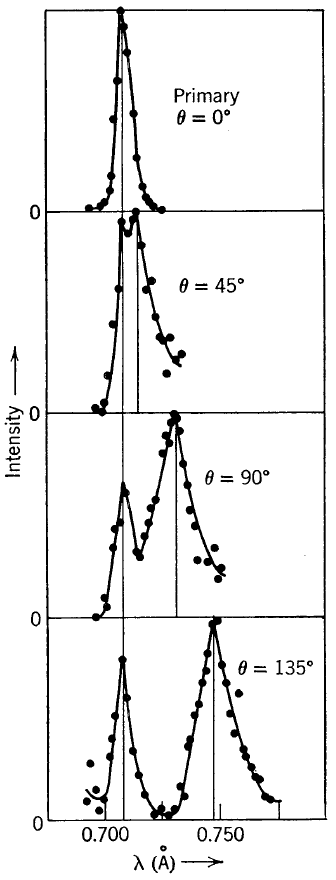
\includegraphics[scale=.8]{compton_exp_data.png}
%% http://hyperphysics.phy-astr.gsu.edu/hbase/quantum/compdat.html#c1
\caption{Compton'un deney sonuçları \cite{book:EisbergResnick}. $0^\circ$'den $135^\circ$ dereceye kadar çizilen çizgi gelen fotonun dalga boyunu ($\lambda$), diğer çizgiler ise saçılan fotonun dalga boyunu ($\lambda'$) göstermektedir.}
\label{fig:compton_exp}}
%%%%%%%%%%
\noindent\rule{.98\textwidth}{0.4pt}
%%
denklemi elde edilir. Bu denklem yeniden düzenlenerek saçılan elektronun momentumu bulunabilir,
\begin{align}
\label{eq:compton_E_conv4}
p_{e'}^{\, 2}c^2 = (h\nu - h\nu' + m_{e}c^2)^2-m_{e}^2c^4.
\end{align}
%%
\end{minipage}
%%
%%
\hspace{12pt}
%%
%%
\begin{minipage}{0.54\textwidth}
{\center
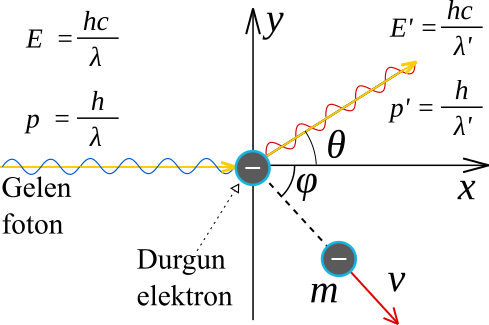
\includegraphics[scale=1.2]{Compton_effect_illust.png}
\caption{Serbest (veya zayıf bağlı) ve durgun bir elektrona gelen bir fotonun saçılmasının parçacık modeline göre temsili.}
\label{fig:compton_duzenek}}
%%%%%%%%%%

\vspace{12pt}

%%%%%%%%%%
\noindent\rule{.98\textwidth}{0.4pt}
%%
Momentumun korunumunu belirleyen Denk. \ref{eq:compton_E_conv2} yeniden düzenlenirse,
%%
\begin{align}
\label{eq:compton_E_conv5}
\vec{p}_{e'} = \vec{p}_\gamma - \vec{p}_{\gamma'}
\end{align}
%%
halini alır. Saçılan elektronun momentumunun kendisiyle iç (skaler) çarpımı sonucunda,
\begin{align}
\label{eq:compton_E_conv6}
p_{e'}^{\, 2} &= \vec{p}_{e'}\cdot\vec{p}_{e'} = (\vec{p}_\gamma - \vec{p}_{\gamma'}) \cdot (\vec{p}_\gamma - \vec{p}_{\gamma'}) \\
 &= p_{\gamma}^{\, 2} + p_{\gamma'}^{\, 2} - 2 p_{\gamma}\, p_{\gamma'} \cos\theta. 
\end{align}
elde edilir. Elde edilen son eşitliğin her iki tarafı $c^2$ ile çarpılır ve foton momentumları yerine $p = E/c = h\nu$ yazılabileceği hatırlanırsa,
%%
\begin{align}
\label{eq:compton_E_conv7}
p_{e'}^{\, 2}c^2 = p_{\gamma}^{\, 2}c^2 + p_{\gamma'}^{\, 2}c^2 - 2c^2 p_{\gamma}\, p_{\gamma'} \cos\theta \nonumber \\
p_{e'}^{\, 2}c^2 = (h \nu)^2 + (h \nu')^2 - 2(h\nu)(h \nu')\cos{\theta}
\end{align}
%%
eşitlikleri elde edilir. Denk. \ref{eq:compton_E_conv4} ve  \ref{eq:compton_E_conv7}'nin sol tarafları eşit olduğuna göre sağ tarafları da birbirine eşit olmalıdır. Bu durumda,
%%
\begin{align}
\label{eq:compton_E_conv8}
(h\nu - h\nu' + m_e c^2)^2 - m_e^{\, 2}c^4 = \nonumber\\
= \left(h\nu\right)^2 + \left(h \nu'\right)^2 - 2h^2 \nu\nu'\cos{\theta}
\end{align}
%%
olur. Gerekli sadeleştirmeler yapılırsa,
%%
\begin{align}
\label{eq:compton_E_conv9}
2 h \nu m_e c^2-2 h \nu' m_e c^2   = 2 h^2 \nu \nu' \left( 1 - \cos \theta \right)
\end{align}
olur. Her iki taraf $ 2h\nu\nu'm_e c$ ile sadeleştirilirse ve $\nu = c/\lambda$ olduğu hatırlanırsa,
%%
\begin{align}
\label{eq:compton_E_conv10}
\lambda'-\lambda = \frac{h}{m_ec}(1-\cos{\theta})
\end{align}
dalga boyundaki kaymayı veren denklem elde edilmiş olur. $h/m_e c \eqsim 2.4\times10^{-10} cm$ değerindedir ve elektronun Compton dalga boyu olarak adlandırılır.

\end{minipage}
\end{figure}


\subsection{Parçacık mı, Dalga mı?}

1923'te {\it Louis de Broglie} ``Işık paketinin geçici teorisi" adlı çalışmasında her ışık paketinin eylemsiz kütlesinin $m_0$ olması gerektiğini ve
bu kütle çok küçük olduğundan ışık paketinin (fotonun) hızının neredeyse ışık hızı $c$ çok yakın olması gerektiğini öne sürmüştür. Böylece bir fotonun bütün enerjisi için,
\begin{equation}
\label{eq:foton_deBroglie_E}
h \nu = \frac{m_0 c^2}{\sqrt{1-v^2/c^2}}
\end{equation}
eşitliğini önermiştir \cite{book:FrenchAP}. Bu eşitlikten yola çıkarak hafif kütleli bütün parçacıklar için,
\begin{equation}
\label{eq:deBroglie_P}
\lambda = \frac{h}{p}
\end{equation}
olacağını öne sürdü. de Broglie fotonu hafif de olsa kütleli kabul etmiştir, fakat günümüzde fotonun kütlesinin sıfır olduğu kabul edilmektedir. de Broglie'nin asıl katkısı bu formülüne getirdiği yeni yorumdur. Bu yoruma göre ışık paketi {\it dalga-parçacık} ikilik (dualite) doğasına sahipse kütleli parçacıklar da {\it parçacık-dalga} ikilik doğasına sahip olmalıydı. 

Örneğin elektron parçacığı de Broglie'nin önerdiği ifadeyle hesaplanan bir dalga boyuna sahip bir dalga gibi davranabilirdi. Bu öneriye ilk deneysel destek C. J. Davisson ve L. H. Germer tarafından gerçekleştirilen elektron kırınımı (difraksiyonu) deneyinden gelmiştir. 

%%
\begin{figure}[hbtp]
\center
\begin{minipage}{0.45\textwidth}
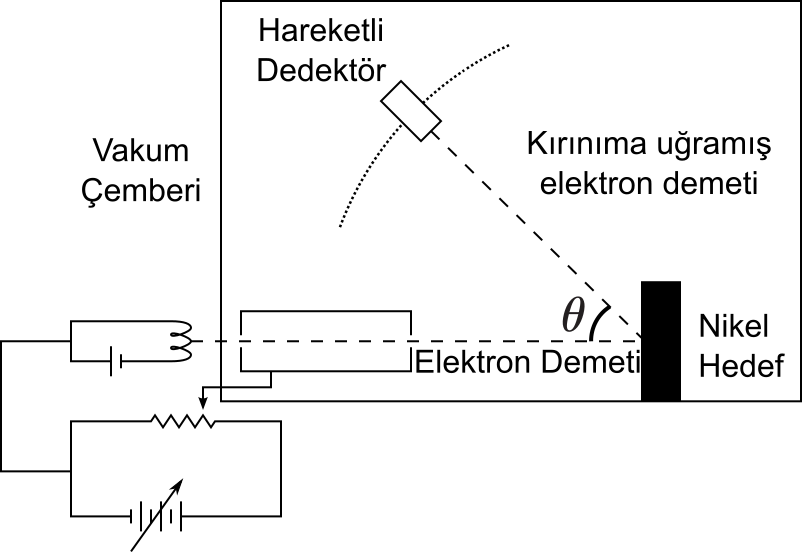
\includegraphics[scale=.7]{Davisson-Germer_experiment.png}
\caption{Davisson ve Germer'in deney düzeneğinin şeması\cite{web:wiki_davisson_germer1}.}
\label{fig:davisson_germer1}
\end{minipage}
%%%
\hspace{24pt}
%%%
\begin{minipage}{0.45\textwidth}
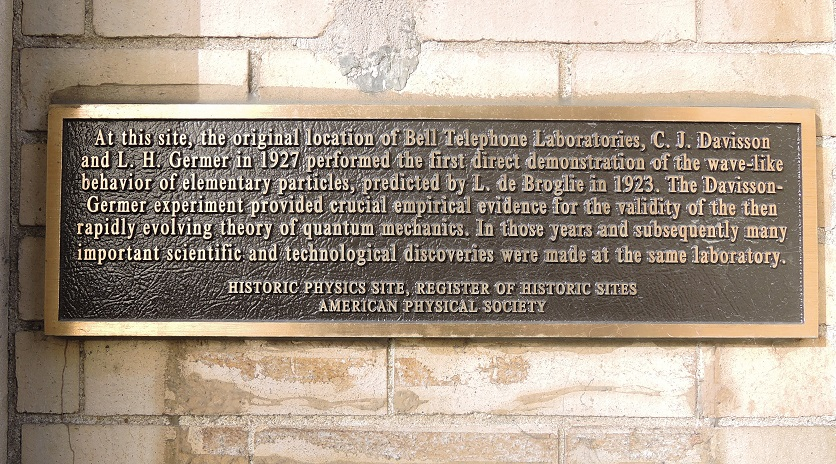
\includegraphics[scale=.35]{Bell_Labs_APS_plaque_west_side_of_Westbeth_door_jeh_edited.jpg}
\caption{Davisson ve Germer'in anısına düzenlenen deneyin gerçekleştirildiği Bell laboratuvarındaki anı tablosu\cite{web:wiki_davisson_germer1}.}
\label{fig:davisson_germer2}
\end{minipage}
\end{figure}

Davisson ve Germer Şekil \ref{fig:davisson_germer1}'deki deney düzeneğinde hızlarını belirledikleri elektron demetlerini Nikel kristal hedefe göndererek deneylerini gerçekleştirmişlerdir. Bu hedef Şekil \ref{fig:davisson_germer4}'teki gibi bir geometrik yapıya ve Şekil \ref{fig:davisson_germer3}'teki bir kristal yapıya sahiptir. Uygun momentuma sahip elektronlar şekildeki gibi bir kristal yapıdan saçıldıklarında eğer dalga özelliğine sahiplerse yıkıcı ve yapıcı girişimler yapacaklardır. Bu durumda kısmen Bragg yasasına uyarlar. Böylece Şekil \ref{fig:davisson_germer5}'da verilen denklemlere göre kırınıma uğrayıp yapıcı girişim yapan elektronların dalga boyları bulunabilir. Davisson ve Germer'in deneyinde elde edilen sonuçlar Şekil \ref{fig:davisson_germer4}'ün alt kısmında görülmektedir. Bragg yasasıyla ilişkili olarak elektronların dedektörde gözlenen şiddetlerinin davranışları anlaşılabilir.

Davisson ve Germer'den sonra ise moleküler hidrojen, helyum ve yavaş nötronlarla da benzeri deneyler gerçekleştirilmiş ve parçacıkların dalga yapısındaki davranışları tekrar tekrar gözlenmiştir \cite{book:Gasiorowicz}.

Çok küçüklerin dünyasında (mikroskopik seviyede) dalga davranışını gözlemek mümkünken, büyüklerin dünyasında (makroskopik seviyede) dalga davranışını gözlemek mümkün değildir. Örneğin, 0.1 mm yarıçaplı, $4\times 10^{-3}$~mg kütleli ve 10 cm/s ile ilerleyen bir su damlası için De Broglie dalga boyu,
%%
\begin{equation*}
\lambda = h/p = 6.6\times 10^{-27} \text{[erg s]}\,/\,(4\times 10^{-5} \text{[g cm/s]}) \eqsim 1.6\times 10^{-22}\,\text{cm}
\end{equation*}
%%
iken, Proton'un yarı çapı $10^{-13}$~cm'dir. Bu nedenle günlük yaşantımızda ve deneylerimizde makroskopik seviyede dalga etkilerini gözleyemeyiz \cite{book:Gasiorowicz}. Işığın veya elektromanyetik dalganın parçacık yapısı davranışının gözlenebilmesi için ise ışığın paketinin dalga boyu ve momentumunun çarpımı Planck sabiti civarında olmalıdır ($\lambda p \eqsim h$).


\begin{figure}[hbtp]
\center
\begin{minipage}{0.45\textwidth}
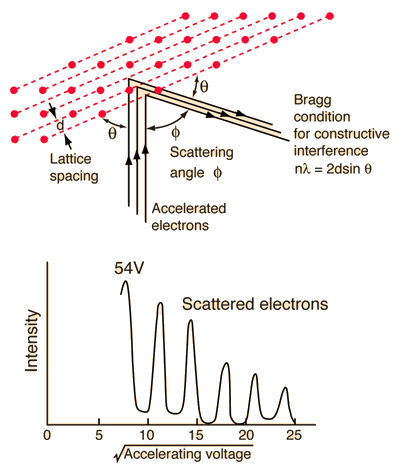
\includegraphics[scale=.8]{davisson_germer_hyperphysics.png}
\caption{Davisson ve Germer'in deney sonuçları\cite{web:hyperphysics_davisson_germer1}.}
\label{fig:davisson_germer3}
\end{minipage}
%%%
\hspace{24pt}
%%%
\begin{minipage}{0.35\textwidth}
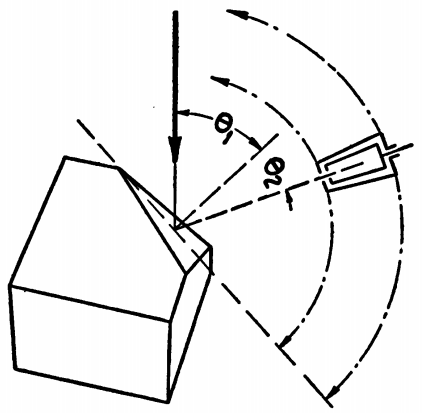
\includegraphics[scale=.35]{Davisson-Germer_experiment_nickel_target.png}
\caption{\label{fig:davisson_germer4} Deneyde kullanılan hedefin geometrik yapısı \cite{DavissonGermer}. Kalın ok gelen elektron demetlerini temsil etmektedir.}

\vspace{24pt}

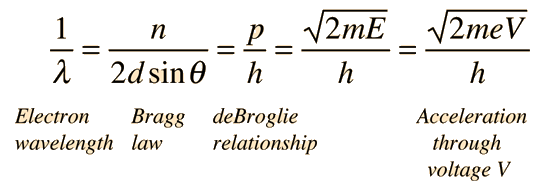
\includegraphics[scale=.4]{davisson_germer_hyperphysics_bragg.png}
\caption{\label{fig:davisson_germer5} Deney sonuçlarının Bragg yasası ile ilişkisi \cite{web:hyperphysics_davisson_germer1}.}
\end{minipage}
\end{figure}


\vspace{24pt}

{\bf Çift yarık deneyi sonra yazılacak...}

\href{https://tr.wikipedia.org/wiki/%C3%87ift_yar%C4%B1k_deneyi}{Bu linkten okunabilir. }
%% https://tr.wikipedia.org/wiki/Çift_yarık_deneyi

\begin{figure}[hbtp]
\center
\begin{minipage}{0.45\textwidth}
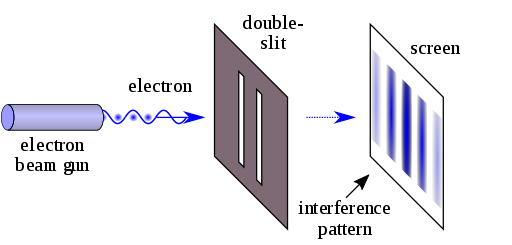
\includegraphics[scale=.4]{Double-slit.png}
\caption{Tonomura \cite{web:wiki_double_slit_experiment}.}
\label{fig:tonomura}
\end{minipage}
\begin{minipage}{0.45\textwidth}
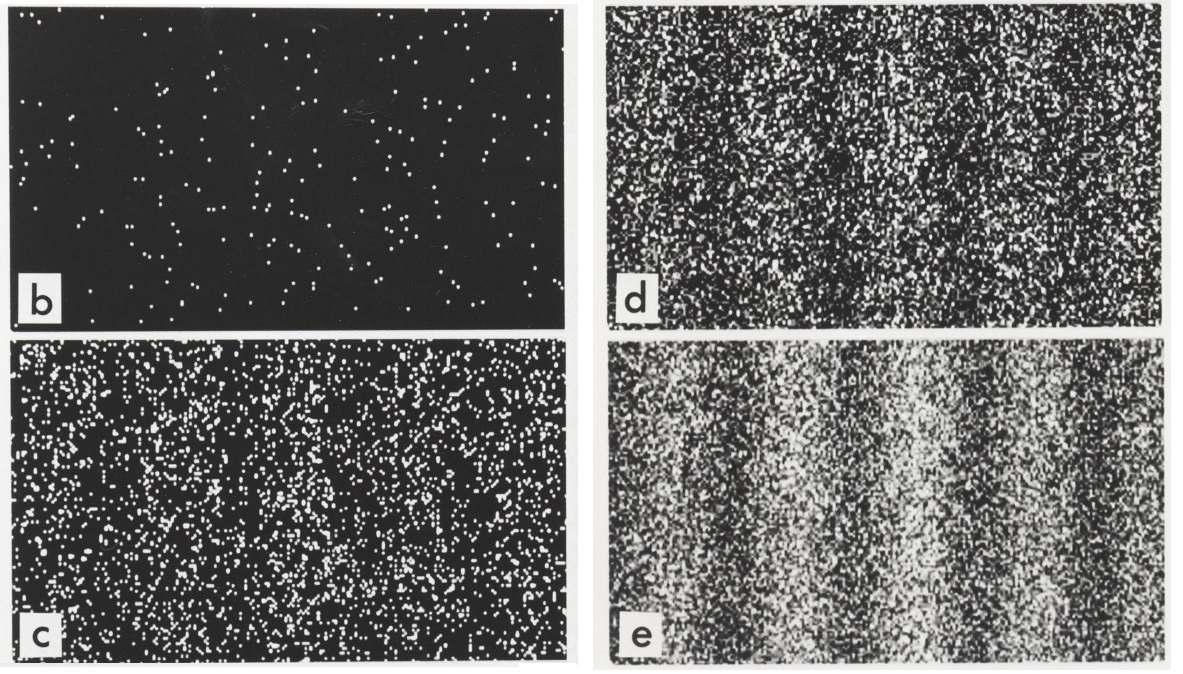
\includegraphics[scale=.8]{Double-slit_experiment_results_Tonomura_2.jpg}
\caption{Tonomura \cite{web:wiki_double_slit_experiment}.}
\label{fig:tonomura1}
\end{minipage}
\end{figure}

\newpage

\subsection{Rutherford ve Bohr Atom Modelleri}

\begin{figure}[hbtp]
\center
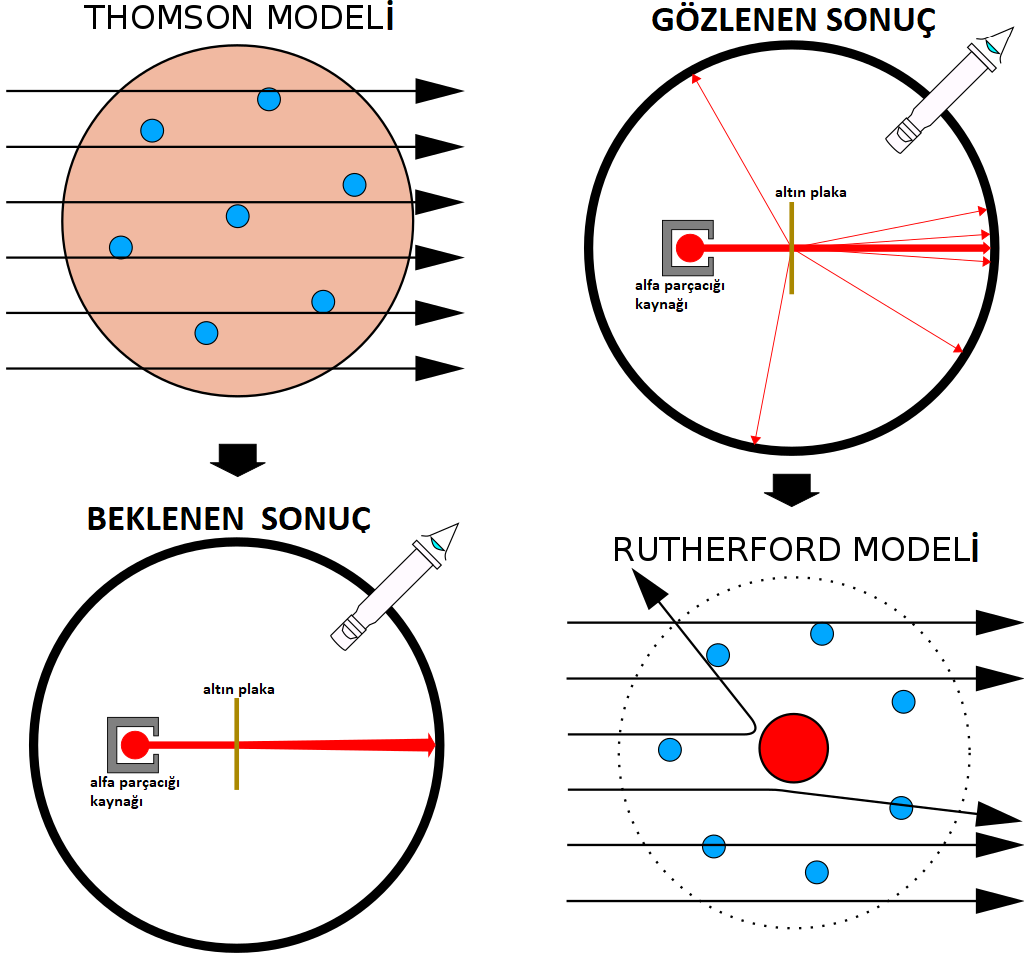
\includegraphics[scale=.5]{Thomson_vs_Rutherford_Atom.png}
\caption{ {\it Solda:} Thomson tarafından önerilen atom modeli ve bu modele göre alfa saçılım deneyinin beklenen sonucu. {\it Sağda:} Gerçekleştirilen deneydeki sonuç ve bu sonuca göre Rutherford'un önerdiği gezegen atom modeli. }
\label{fig:rutherfod_bohr_atom}
\end{figure}

Henri Becquerel ve Marie Cruie'nin öncülüğüne yaptığı radyoaktivite çalışmaları sonucunda, atomun iç yapısını çalışmak için gerekli araçlar ortaya çıkmış oldu. Bunlardan birisi ilk önceleri $\alpha$ (alfa) parçacıkları olarak adlandırılmış parçacıklardır, çok daha sonra helyum atomunun çekirdeği olduğu anlaşılmıştır. 

Ernest Rutherford'un gözetiminde H. W. Geiger  ve E. Marsden tarafından 1908'de altın bir plakadan alfa parçacıklarının saçılımı deneyleri gerçekleştirilmiştir. Şekil \ref{fig:rutherfod_bohr_atom} temsili gösterilen Thomson atom modeline göre gerçekleştirilen deneylerin sonucunda alfaların çok küçük açılarla saçılacakları öngörülebilir. Çünkü elektronun kütlesi alfa gibi büyük kütleli bir parçacığın büyük açılı saçılmalaya uğraması için yeterli değildir. Modele göre elektronları çevreleyen pozitif bulut (!) ise gerekli saçılmayı sağlayacak kadar yoğun değildir.

Fakat deneylerde nadiren de olsa, Şekil \ref{fig:rutherfod_bohr_atom}'da görüldüğü üzere, büyük açılı saçılmaların gerçekleştiği gözlenmiştir. Deneylerin ayrıntılı tarihçesine {\it \href{https://history.aip.org/exhibits/rutherford/sections/alpha-particles-atom.html}{Alpha Particles and the Atom}} başlıklı web sayfasından ulaşılabilir \cite{web:rutherford_bohr_atom}. Rutherford deney sonuçlarına göre gezegen atom modeli olarak da isimlendirilen atom modelini önermiştir. Bu modele göre pozitif yükler atomun merkezinde ve çok küçük bir hacimde toplanmış olmalıdır. Böylece alfa parçacıkları büyük kütleli bir merkezden daha büyük bir itici potansiyelle saçılırlar. Bu atom modeline göre elektronlar büyük kütleli ve pozitif yüklü bu merkez etrafında $1/r^2$ ile orantılı çekici bir kuvvet etkisinde dairesel veya eliptik yörüngeler izlerler.

Rutherford atom modeliyle büyük açılı alfa saçılmaları açıklanabilmiş, fakat yeni sorunlar ortaya çıkmıştır. Elektronlar atom çekirdeği etrafında dairesel yörüngede dönerken, merkezcil bir ivmeyle, ivmeli hareket yaparlar. Klasik elektrodinamik (KED) teoriye göre ivmeli hareket yapan her elektrik yüklü parçacık ışıma yapar. Bu durumda elektronların nasıl kararlı yörüngelere sahip oldukları açıklanamaz. Çünkü ışıma yapan elektronların enerji kaybederek ve spiral bir yörünge izleyerek \href{http://bcs.wiley.com/he-bcs/Books?action=mininav&bcsId=1533&itemId=0471057002&assetId=17327&resourceId=1342}{10$^{-10}$~s}'de çekirdeğe düşmeleri beklenir. Dahası KED'eye göre yayınlanan ışınımın frekansı elektronun periyodik hareketinin frekansı ile aynı olmalıydı. Fakat, o zamana kadar elde edilen atomik spektrum bilgileriyle bu sonuç çelişmekteydi. Anders Angstrom ve diğerlerinin sonuçlarını inceleyen Swiss Johann Balmer 1885'de ışımaların dalga boyunu veren, 
%%
\begin{equation}
\frac{1}{\lambda}= R_y \left( \frac{1}{n_1^2} - \frac{1}{n_2^2} \right)
\label{eq:balmer}
\end{equation}
formülünü keşfetti. Burada $n_1$ ve $n_2$ tam sayı, $R_y$ bir sabittir \cite{book:Gasiorowicz}.

Neils Bohr 1913 yılında, Rutherford'dan iki yıl sonra, bu çelişkileri ortadan kaldırabilmek için kendi varsayımlarını fizik topluluğu ile paylaştı. Bu varsayımlar klasik fiziğin sınırları dışında kalmakla beraber belli ölçüde Rutherford atom modelindeki çelişkilere cevap verdiği düşünülebilir. Çünkü spektrumu açıklarken, kararlılık problemi üzerinde durmamıştır.

\begin{itemize}
\item Bir atomik sistemin varlığı ancak {\it kesikli durağan seviyeler} ile izah edilebilir. Buna göre sistemdeki herhangi bir enerji değişikliği böyle iki seviye arasındaki tam geçişlerle mümkün olabilir.

\item İki durağan seviye arasındaki geçişler sırasında yayınlanan veya soğurulan elektromanyetik ışınımın frekansı seviyelerin enerjileri $E_1$ ve $E_2$ ile,
\begin{equation}
h\nu = E_2 - E_1
\label{eq:bohr_states}
\end{equation}
şeklinde doğrudan ilişkilidir.

\item Bu durağan seviyeler Rutherford atom modelindeki izinli yörüngelere (orbitlere) karşılık gelirler. Bu yörüngelerde elektronlar klasik fizikteki gibi herhangi bir açısal momentum değerini alamazlar, bunun yerine açısal momentumları
\begin{equation}
L = m v r  = n \frac{h}{2 \pi}
\label{eq:bohr_allowed_states}; \;\;\;\; n=1,2,3, \dots
\end{equation}
ifadesine uyan ve tam sayılarla ifade edilen yörüngelerede bulunabilirler.
\end{itemize}

\begin{figure}[hbtp]
\center
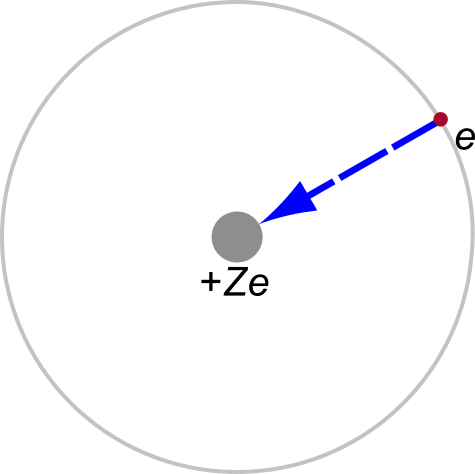
\includegraphics[scale=.8]{Bohr-atom-PAR.png}
\caption{Bohr ve Rutherford atom modeline göre tek elektronlu bir atomik yapının temsili.}
\label{fig:bohr_atom}
\end{figure}

Bu varsayımlardan elde edilen teorik sonuçlar hidrojen gibi tek elektronlu ve dairesel yörüngeli atomları izah etmede başarılı olmuştur. Şekil \ref{fig:bohr_atom}'deki temsile göre elektron üzerinde Coulomb yasası gereğince,
%%
\begin{equation}
F_e = \frac{1}{4\pi\varepsilon_0} \frac{Ze^2}{r^2}
\label{eq:bohr_elektron}
\end{equation}
%%
çekici kuvveti oluşur. Klasik olarak Newton mekaniğinde bir cisme dışarıdan uygulanan merkezcil kuvvetler için,
%%
\begin{equation}
\sum F_\text{dış} = m_e a = m_e v^2/r
\label{eq:newton_ma}
\end{equation}
%%
yazılabilir. Elektrona uygulanan tek merkezcil ve dış kuvvet Coulomb kuvveti olduğuna göre elektronun hareketini betimlemek için,
%%
\begin{equation}
\frac{1}{4\pi\varepsilon_0} \frac{Ze^2}{r^2} = \frac{m_e v^2}{r} 
\label{eq:bohr_orbit_motion}
\end{equation}
%%
yazılabilir. Bohr'un açısal momentum ile ilgili varsayımı (Denklem \ref{eq:bohr_allowed_states}) elde edilen bu son eşitlikte kullanılırsa, sırasıyla elektronun yörünge sürati ve yörünge yarı çapı,
%%
\begin{equation}
v = \frac{Ze^2}{4\pi\varepsilon_0}  \frac{2\pi}{n h}
\label{eq:bohr_elektron_speed}
\end{equation}
%%
ve
%%
\begin{equation}
r = \left(\frac{n h}{2 \pi} \right)^2 \frac{1}{m_e}\, \frac{1}{(Z e^2/4\pi\varepsilon_0)}
\label{eq:bohr_elektron_radius}
\end{equation}
%%
olur. Klasik olarak elektronun toplam enerjisi,
%%
\begin{equation}
E = \frac{1}{2}m_e v^2 - \frac{Z e^2}{4\pi\varepsilon_0 r}
\label{eq:bohr_elektron_energy1}
\end{equation}
%%
ifadesi ile tanımlanır. Bohr'un modelinden elde edilen sürat ve yarıçap bu denklemde yerine konursa,
%%
\begin{equation}
E = -\frac{1}{2} \left(\frac{2\pi}{h} \right)^2 \left(\frac{Ze^2}{4\pi \varepsilon_0} \right) \frac{1}{n^2}
\label{eq:bohr_elektron_energy2}
\end{equation}
%%
elektronun toplam enerjisi olarak bulunur. Bu sonuç, Bohr'un elektronların yörünge geçişlerinde yayınlanan elektromanyetik dalganın enerjisini tanımlayan varsayımı ile birleştirildiğinde, Balmer tarafından önerilen (Denk. \ref{eq:balmer}) seviye geçişleri denklemine ulaştırır.

Elektronun enerjisi, sürati ve yarıçapı için yukarıda elde edilen ifadeler bir kaç yeni tanımla daha pratik yazılabilirler. İndirgenmiş Plank sabiti 
%%
\begin{equation}
\hbar = \frac{h}{2\pi} = 1.054571800 \times 10^{-34}\ \text{J}\,\text{s}/\text{rad}
\label{eq:reduced_planck_const}
\end{equation}
%%
olarak tanımlanırsa ve $\nu$ (frekans) yerine $\omega = 2\pi \nu$ (açısal frekans) kullanılırsa Denk. \ref{eq:bohr_states}, 
%%
\begin{equation}
\omega = \frac{E_2 - E_1}{\hbar}
\label{eq:bohr_states_2pi}
\end{equation}
%%
halini alır. Benzer şekilde, elektromanyetik ışıma paketinin (fotonun) enerjisi,
%%
\begin{equation}
E = \hbar \omega
\label{eq:foton_energy_2pi}
\end{equation}
%%
olarak yazılabilir. Bohr'un açısal momentum varsayımı,
%%
\begin{equation}
m v r = n \hbar
\label{eq:bohr_allowed_states_2pi}
\end{equation}
%%
şeklinde yeniden yazılabilir. Ayrıca ``ince yapı sabiti" adı verilen pratik bir sabit de çok sık kullanılır. Bu sabit ise,
%%
\begin{equation}
\alpha = \frac{e^2}{4\pi\varepsilon_0\hbar c} =\frac{1}{137.036}
\label{eq:fine_structure_const}
\end{equation}
%%
olarak tanımlanmıştır. Bu yeni tanımlarla sürat, yarı çap ve enerji ifadeleri sırasıyla,
%%
\begin{equation}
v = \frac{Z \alpha c}{n} \hspace{24pt} r = \frac{\hbar}{m_e c Z \alpha} n^2
\label{eq:bohr_v_r_2pi}
\end{equation}
%%
ve
%%
\begin{equation}
E = -\frac{1}{2}m_e (Z \alpha c)^2 \frac{1}{n^2}
\label{eq:bohr_E_2pi}
\end{equation}
%%
olarak yazılırlar. Bu ifadelerle Şekil \ref{fig:bohr_atom}'deki gibi herhangi bir tek elektronlu atom için,

\begin{itemize}
\item en düşük yörüngenin (n=1) yarı çapı (Bohr yarı çapı olarak da adlandırılır),
\begin{equation}
a_0 = \frac{\hbar}{m_e c Z \alpha} 1^2 \eqsim \frac{137\hbar}{m_e c Z} = \frac{0.053}{Z}\times 10^{-9} \text{m} = \frac{0.053}{Z} \text{nm} = \frac{0.53}{Z} \text{\AA}
\label{eq:bohr_radius}
\end{equation}

\item en düşük Bohr yörüngesindeki elektronun bağlanma enerjisi ve koparma enerjisi (elektronun serbest hale gelmesi için gerekli enerji),
%%
\begin{eqnarray}
\text{Bağlanma Enerjisi} &\equiv& E(n=1) = -\frac{1}{2}m_e (Z \alpha c)^2 \frac{1}{1^2} \eqsim -13.6 Z^2 \text{eV} \\
\text{Koparma Enerjisi} &\equiv& E(n\rightarrow\infty) - E(n=1) = 0 - (-13.6 Z^2) = 13.6 Z^2 \text{eV}
\label{eq:bindingEnergy}
\end{eqnarray}
\end{itemize}
%%
olarak bulunur. Böyle bir atoma hidrojen (Z=1) örnek verilebilir, hidrojenin atomunun elektronu n=2 seviyesinden n=1 seviyesine geçişi sırasında elektromanyetik ışınım (foton) yayınlayarak enerji kaybeder. Elektronun kaybettiği enerji veya yayınlanan ışınımın enerjisi,
%%
\begin{eqnarray}
\text{Fotonun Enerjisi} &\equiv& E(n=2) - E(n=1) 
= -\frac{13.6}{2^2} - (-\frac{13.6}{1^2}) \nonumber \\ 
&=&  13.6 (1-\frac{1}{4}) \text{ eV} = 10.2 \text{ eV}
\label{eq:fotonEnergy}
\end{eqnarray}
%%
olacaktır. Yayınlanan fotonun açısal frekansı ise Denk. \ref{eq:bohr_states_2pi}'e göre,
%%
\begin{equation*}
\omega = \frac{E_2 - E_1}{\hbar} = \frac{10.2 \text{ eV}}{6.58\times 10^{-16} \text{ eV s/rad}} \eqsim 1.6 \times 10^{16} \text{ rad/s}
\end{equation*}
%%
dir. Aynı fotonun dalga boyu ise,
%%
\begin{eqnarray*}
E &=& \hbar \omega = \hbar 2\pi \nu = \hbar 2\pi c/\lambda, \\
\lambda &=& \frac{\hbar 2\pi c}{E} = 
\frac{6.58\times 10^{-16} \text{ eV s/rad } 2\pi\,3\times 10^8 \text{m/s}}{10.2 \text{eV}}\eqsim 1.2\times 10^{-7} \text{m}\\
\lambda &=& 120 \text{ nm} = 1200 \text{ \AA} 
\end{eqnarray*}
olarak bulunur. Bu ışınım elektromanyetik spektrumun morötesi kısmında yer alır ve deneysel verilerle uyumludur. Böylece daha önce anlaşılamayan deneysel bazı sonuçlar Bohr atom modeli ile aydınlatılabilmiştir. Bohr modeli önemli bir başarı gösterse de, elektronlar ne zaman bir yörüngeden sıçrama yapmalı veya yayınlanan fotonun yönü ne olmalı gibi sorulara yanıt verememiştir. Ayrıca açısal momentumun ve seviyelerin kuantumlanma kuralı sadece dairesel yörüngeli durumlar için geçerlidir. Eliptik yörüngeler için A. Sommerfeld ve W. Wilson bir başka kuantumlanma şartı tanımlamışlardır \cite{book:Gasiorowicz, book:EisbergResnick}. 
%%

\vspace{12pt}

\href{http://hyperphysics.phy-astr.gsu.edu/hbase/FrHz.html}{Franck-Hetz deneyi.... }


\subsection{Uygunluk İlkesi}
\href{http://hyperphysics.phy-astr.gsu.edu/hbase/quantum/hosc6.html}{uygunluk ilkesi}









\newpage
% In the preamble, add "\renewcommand\refname{New Title}" for article type documents 
% and "\renewcommand\bibname{New Title}" for book and report type documents.
\renewcommand\refname{Kaynaklar}
\bibliography{quantumBIB}{}
%% https://www.sharelatex.com/learn/latex/bibtex_bibliography_styles
 \bibliographystyle{plain}
%% \bibliographystyle{alpha}
%%\bibliographystyle{apalike}
\end{document}

